% \documentclass[../../Orator]{subfiles}
\documentclass[class={myRUCProject}, crop=false]{standalone}

\IfStandalone{%
    \usepackage[disable]{todonotes}
    \import{../../}{customCommands}
    \import{../../}{INP-00-glossary}
    }{}

    
\usepackage{myTikz}
\usepackage{halloweenmath}
    
\begin{document}

The colossal size of the squid axon initially led to the misconception, where it was believed to be associated with the animal's blood vessel structure. The field of neuroscience is actually indebted to zoologist J. Z. Young, by bringing the squid giant axon, in 1939, to the forefront, by highlighting it as a valuable experimental model for investigating the mechanisms behind the cellular membrane of the neurons. Hodgkin and Huxley utilized this experimental setup and decoded the ionic framework of action potential, and even today, the giant axon remains an ongoing cornerstone in a diverse spectrum of investigations \cite{wood1996neuroscience}. 
The circuit for the Hodgkin-Huxley model can be seen in \Cref{fig:HHcircuit}. 

\begin{figure}[ht]
    \centering
    \import{../../Pictures/Anakin}{HoHu.tex}
    \caption{The equivalent \gls{gls:circuit} of the \gls{hh} model for a short segment of squid giant axon. The capacitor represents the capacitance of the cell membrane; the two variable resistors represent voltage-dependent \gls{Na} and \gls{K} conductances, the fixed resistor represents a voltage-independent leakage conductance and the three batteries represent reversal potentials for the corresponding conductances. The pathway labeled “stim” represents an externally applied current, such as might be introduced via an intracellular electrode.~\cite{HodHux1952}.}\label{fig:HHcircuit}
\end{figure}


The \gls{hh} model of \gls{ap} is an ion channel model \cite{Valle2022} of a large squid axon being \gls{gls:nonlinear}. It is based on the electrical properties of the membrane where it describes the generation and propagation of action potentials, by approximating the characteristics of excitable cells, such as neurons, to a circuit-like construct \cref{fig:MembraneCircut}\cite{ChuangChung}. It deals with a system of differentiable equations with four state variables \(\unit{\V\membrane}\of{t}, \ n\of{t}, \ m\of{t}, \ h\of{t}\) with respect to time \cite{HodHux1952}. It exploits the space- and voltage-clamp methods to collect parameter values, whose extraction is a complicated but principal attribute in neuroscience \cite{Valle2022}. 
Recall that \cref{eq:nasum, eq:ksum} gives the relationship of unitary currents to total current for their respective ions, using similarities one can restate the equations more generally as:
\begin{align}
 \curr\ion&= N \, p_o \, \ucur\ion \label{eq:curgen}\\
\intertext{By analogy, the total \gls{gls:admit} of the \gls{gls:membrane} for a particular \gls{gls:ion} is: }
 \unit{\cond\ion} &= N \, p_o \, \ucon\ion \label{eq:congen}\\
\intertext{substituting \cref{eq:congen,eq:curgen} into \cref{eq:cur2con} gives us:}
 \curr\ion &= \unit{\cond\ion} \, \br{\unit{\V} - \equi\ion}\label{eq:ionCurrent}
\end{align}
In the \textit{\gls{gls:space-clumping}} HH model, the voltage is being maintained at a constant level, allowing for the examination of membrane properties as though they were uniform across the entire neuronal length. This is carried out to facilitate the investigation of the character of ionic channels and the cellular membrane despite challenges associated with structural voltage alterations. The flow of current is represented mathematically, as the change in voltage over time scaled by capacitance.
    \begin{equation}
        \capa\membrane \ode{\unit{\V\membrane}} + \curr\ion  = \curr\total
    \end{equation}
where \(I\total\) is the total current imposed on the cellular membrane, \(C\membrane\) is the membrane capacitance per unit area. Recall, in \Cref{eq:ionCurrent}, that the current through a given \gls{gls:ionChan} \(\curr\ion\) is the product of that channel's \gls{gls:contan} and the \gls{gls:rPote} for the specific ion
    \begin{equation}
        \curr\ion = {g_\bfm{ion}}(\unit{\V\membrane}-\unit{\V\ion})  
    \end{equation}
where \(\unit{\V\ion} = \equi\ion = \equi\reverse\). Thus, for a cell with \gls{Na} and \gls{K} channels, the total current through the membrane can be defined by:
\begin{equation}
     \curr\total  = \capa\membrane \ode{\unit{\V\membrane}} + \curr\ion = \capa\membrane \ode{\unit{\V\membrane}} + \sum\ion^{i} I_i = \curr_\rmm{ext} + \sum\ion^{i} \sbr{\cond_i \br{\unit{\V\membrane}-\unit{\V_i}}} 
\end{equation} 
with \(\curr\ion\) representing the total membrane current per unit area; %\quad C\membrane \ode{\unit{\V\membrane}}
\begin{alignat}{5}
    &\quad \curr\ion &&= \quad \curr\potassium \quad&&+ \quad \curr\sodium \quad&&+ \quad \curr\leakage \\ 
    \implies & &&=  \cond\potassium\br{\unit{\V\membrane} - \unit{\V\potassium}} &&+ \cond\sodium \br{\unit{\V\membrane} - \unit{\V\sodium}}  &&+ \cond\leakage \br{\unit{\V\membrane} - V_\rmm{L}} \nonumber
\end{alignat}
\(\cond\potassium\), \(\unit{\V\potassium}\), along with  \(\cond\sodium\), \(\unit{\V\sodium}\) make up the \gls{gls:cond} and \gls{gls:rPote} of \gls{K} and \gls{Na} respectively.
The directly time dependent element of this equation is \(\unit{\V\membrane}\), with \(\cond\sodium\), and \(\cond\potassium\) dependent on both \(\br{\unit{\V\membrane}}\){,} and as described in \Cref{sec:ap}{,} dependent on time as a consequence of \gls{gls:ionChan}.

Through long-term experimentation, the duo of Hodgkin and Huxley divined a model built from the observations of smooth current change as a function of pores (or channels) that were either open or closed. By using a statistical approach, HH determed the voltage-dependent rate of channels being open or closed at a given time in the process~\cite{HodHux1939}. 

The `gating variables' \(n\), \(m\), and \(h\) describe the time dependent kinetics of the voltage, representing 
the \emph{probabilities} of individual \gls{gls:ionChan} subunit activation/inactivation\footnote{\underline{a}ctivation gives \(\alpha\), \underline{b}nactivation gives \(\beta\), really these are the obvious choices},~
 commonly denoted by \(\alpha_p, \, \beta_p : \, p \in \left\{n,m,h\right\}\). 
 are defined such that:
\begin{align}
    \alpha_p\of{\unit{\V\membrane}} &= p_\infty \of{\unit{\V\membrane}} / \tau_p \\
    \beta_p\of{\unit{\V\membrane}}  &= \br{1 - p_\infty \of{\unit{\V\membrane}}} / \tau_p 
\end{align}

With \(p_\infty\) and its complementary probability \(\br{1-p_\infty}\) being the steady state values for activation and inactivation respectively~\cite{HodHux1952}. 
In the original paper by Hodgkin and Huxley, the relationships of \(\alpha_p, \text{ and }\, \beta_p\) were defined by:\\
% for squid axons by hodgkin and huxely
\noindent%  
\vbox{\vspace{-2.0em}\centering
\begin{minipage}[c]{.50\textwidth}
    \centering
    \vspace{0.75em}
    \scalebox{1.1}{\vbox{%
    \begin{equation*}
        \begin{matrix}
        \text{Fraction in the}\\
        \text{\emph{active} state}\\
        p_i\of{t}
        \end{matrix}\quad
        \begin{matrix}
        \underscriptleftarrow{\alpha_p\of{\unit{\V\membrane}}}\\
        \overscriptrightarrow{\beta_p\of{\unit{\V\membrane}}}
        \end{matrix}\quad
        \begin{matrix}
        \text{Fraction in the}\\
        \text{\emph{inactive} state}\\
        1 - p_i\of{t}
        \end{matrix}\quad
    \end{equation*}}}
    \begin{align*}
    p = m &\implies \left\{
    \begin{aligned}
        \alpha\mch \of{\unit{\V\membrane}} &= 0.1 \cfrac{ 25 - V }{\exp{\cfrac{25-V}{10}} - 1} \\
        \beta\mch \of{\unit{\V\membrane}}  &= 4 \, \exp{-\cfrac{V}{18}} 
    \end{aligned} \right. 
    \end{align*}
\end{minipage}
~\hfill~
\begin{minipage}[c]{.45\textwidth}
    \begin{align*}
    p = n &\implies \left\{
    \begin{aligned}
        \alpha\nch \of{\unit{\V\membrane}} &= 0.01 \, \cfrac{ 10 - V }{ \exp{ 10 - V } - 1} \\
        \beta\nch \of{\unit{\V\membrane}}  &= 0.125 \, \exp{-\cfrac{V}{80}} 
    \end{aligned} \right.\\
    p = h &\implies \left\{
    \begin{aligned}
        \alpha\hch \of{\unit{\V\membrane}} &=  0.07 \, \exp{-\cfrac{V}{20}} \\
        \beta\hch \of{\unit{\V\membrane}}  &= { \cfrac{1}{\exp{\cfrac{30 - V}{10}} + 1}}
    \end{aligned} \right.
    \end{align*}
\end{minipage}
}
% \vspace{1.75em}

Where \(\unit{\V} = \unit{\V_{\rmm{rest}}} - \unit{\V\membrane}\) represents the polarization in \unit{\milli\volt}.
In order to characterize the ion-channels, the equations can be fitted to voltage clamp\footnotemark~data.
\footnotetext{An assay that measures the flow of current through a neuronal cell membrane by `clamping' the potential at an unchanging value.}
As a result, H\&H presented the model as a set of four 
% \anakintodo{Make it more clear that they're `emulating' stochasticity} 
inter-dependent \gls{ode}[s] with respect to time.
\begin{system}[HodHuxSys]
    C\mch \ode{\unit{\V\membrane}} &= I\mch - \mathrlap{\sbr{\mcon\potassium n^4 \br{\unit{\V\membrane} - \unit{\V\potassium}} + \mcon\sodium m^3 h \br{\unit{\V\membrane} - \unit{\V\sodium}}  + \mcon\leakage \br{\unit{\V\membrane} - V_\rmm{L}}}}  && \\
    \ode{n} &=  \frac{n_\infty\of{\unit{\V\membrane}}-n}{\tau\nch\of{\unit{\V\membrane}}}  &&\hspace{-3.5em} =\alpha\nch \of{\unit{\V\membrane}} \br{1-n} - \beta\nch \of{\unit{\V\membrane}} n \qquad && \\
    \ode{m} &=  \frac{m_\infty\of{\unit{\V\membrane}}-m}{\tau\mch\of{\unit{\V\membrane}}}  &&\hspace{-3.5em} =\alpha\mch \of{\unit{\V\membrane}} \br{1-m} - \beta\mch \of{\unit{\V\membrane}} m \qquad && \\
    \ode{h} &=  \frac{h_\infty\of{\unit{\V\membrane}}-h}{\tau\hch\of{\unit{\V\membrane}}}  &&\hspace{-3.5em} =\alpha\hch \of{\unit{\V\membrane}} \br{1-h} - \beta\hch \of{\unit{\V\membrane}} h \qquad &&
\end{system}

\begin{table}[H]
    \centering
    \caption{Parameters of the \acrlong{hh} model determined from studies of squids}\label{tab:fuck}
    \begin{tabular}{m{0.15\textwidth} @{}
                    m{0.58\textwidth}  @{}
                    m{0.15\textwidth}} \hline
        Parameters & Significations & Values \\\hline
    \unit{\curr\total}, \unit{\curr\ion} & Total current density applied on a membrane, \newline Ionic current density, sum of \gls{K},\gls{Na}, and leak currents & \qty{0}{\micro\A/cm^2} \newline\unit{\micro\A/cm^2}\\
    \unit{\capa\membrane} & Membrane Capacitance & \qty{1}{\micro\F/cm^2}\\
    \unit{\V\membrane} & Membrane Potential & mV\\
    %t &time & ms\\
    \unit{\mcon\potassium}, \unit{\mcon\sodium}, \unit{\mcon\leakage} & maximal conductance for \gls{K} \newline maximal conductance for \gls{Na} \newline maximal conductance for “leaking” ions & \qty{36}{\milli\mho/cm^2} \newline \qty{120}{\milli\mho/cm^2}\newline\qty{0.3}{\milli\mho/cm^2} \\
    \unit{\V\potassium}, \unit{\V\sodium}, \unit{\V\leakage} & Equilibrium Potential of \gls{K} \newline Equilibrium potential for \gls{Na} \newline Equilibrium potential for “leaking” ions & \qty{12}{mV} \newline \qty{-115}{mV} \newline \qty{-10.613}{mV} \\ \hline
    \end{tabular}
    %n & Proportion of particles in neuron involved with opening of \gls{K} gate & \\
    %m & proportion of particles in neuron affecting opening of \gls{Na} gate & \\
    %h & proportion of particles outside of neuron affecting closing of “2nd” \gls{Na} gate & \\
    %\unit{\alpha\nch} & Voltage dependent rate for \gls{K} ions to enter the cell per ms & \\
    %\unit{\beta\nch} & Voltage dependent rate for \gls{K} ions to exit the cell per ms & \\
    %\unit{\alpha\mch} & Voltage dependent rate for \gls{Na} to enter the cell per ms via the “1st” gate & \\ 
    %\unit{\beta\mch} & Voltage dependent rate for \gls{Na} to exit the cell per ms via the “1st” gate & \\
    %\unit{\alpha\hch} & Voltage dependent rate for \gls{Na} to exit the cell per ms via the “2nd” gate & \\ 
    %\unit{\beta\hch} & Voltage dependent rate for \gls{Na} to enter the cell per ms via the “2nd” gate &
\end{table}

\begin{comment}
    Breaking down the equation we find the following regions:
    \begin{equation*}
        \curr = 
        \overbrace{C\mch \ode{\unit{\V\membrane}}}^{\mathclap{\text{rate of change of voltage scaled by capacitance}}} + 
        \mcon\potassium n^4 \br{\unit{\V\membrane} - \unit{\V\potassium}} + 
        \mcon\sodium m^3 h \br{\unit{\V\membrane} - \unit{\V\sodium}}  + 
        \mcon\leakage \br{\unit{\V\membrane} - V_\rmm{L}} 
    \end{equation*}




    \begin{figure}[h]
        \centering
        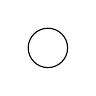
\begin{tikzpicture}
            
            \draw (0,0) circle (0.25);
            
        \end{tikzpicture}
        \caption{fart}\label{<label>}
    \end{figure}
\end{comment}



\end{document}
